\documentclass[a4paper,10pt]{article}

\usepackage[utf8]{inputenc}
\usepackage{t1enc}
\usepackage[spanish]{babel}
\usepackage[pdftex,usenames,dvipsnames]{color}
\usepackage[pdftex]{graphicx}
\usepackage{amsmath}
\usepackage{amsfonts}
\usepackage{amssymb}
\usepackage{listings}
\lstset{language=C}
\lstset{showstringspaces=false}
\lstset{basicstyle=\ttfamily,}

\usepackage{float}
\floatstyle{boxed} 
\restylefloat{figure}

\begin{document}


\renewcommand{\lstlistingname}{C\'odigo Fuente}
\lstloadlanguages{Octave} 
\lstdefinelanguage{MyPseudoCode}[]{Octave}{
	deletekeywords={beta,det},
	morekeywords={repmat}
} 
\lstset{
	language=MyPseudoCode,
	stringstyle=\ttfamily,
	showstringspaces = false,
	basicstyle=\footnotesize\ttfamily,
	commentstyle=\color{gray},
	keywordstyle=\bfseries,
	numbers=left,
	numberstyle=\ttfamily\footnotesize,
	stepnumber=1,                   
	framexleftmargin=0.20cm,
	numbersep=0.37cm,              
	backgroundcolor=\color{white},
	showspaces=false,
	showtabs=false,
	frame=l,
	tabsize=4,
	captionpos=b,               
	breaklines=true,             
	breakatwhitespace=false,      
	mathescape=true
}
\begin{titlepage}
        \thispagestyle{empty}
        \begin{center}
                
\includegraphics{./images/itba.jpg}
                \vfill
                \Huge{Sistemas Operativos}\\
                \vspace{1cm}
                \huge{Trabajo Práctico Especial Nº1}\\
        \end{center}
        \vspace{2cm}
        \large{
                \begin{tabular}{lcrc}
                        \textbf{Alvaro Crespo} & & 50758 & \ \ \texttt{acrespo@alu.itba.edu.ar}\\
                        \textbf{Juan Pablo Civile} & & 50453 & \ \ \texttt{jcivile@alu.itba.edu.ar}\\
                        \textbf{Darío Susnisky} & & 50592 & \ \ \texttt{dsusnisk@alu.itba.edu.ar}\\
                        \\ 
                \end{tabular}
        }
        \vfill
        \flushright{12 de Septiembre del 2011}
\end{titlepage}

\setcounter{page}{1}

\tableofcontents
\newpage
\section{Introducción}
El objetivo de este trabajo es familiarizarse con el uso de sistemas cliente-servidor concurrentes, implementando el servidor mediante la creación de procesos hijos 
utilizando \textit{fork()} y mediante la creación de \textit{threads}. Al mismo tiempo, ejercitar el uso de los distintos tipos de primitivas de sincronización y 
comunicación de procesos (IPC) y manejar con autoridad el \textit{filesystem} de Linux desde el lado usuario.

\newpage
\section{Esquema de la aplicación}

A la hora de encarar el problema en cuestión, una de las primeras cosas a plantearse era el diseño de la aplicación. Dada la naturaleza y los objetivos planteados para este
 trabajo práctico, era necesario poder identificar que partes de nuestra simulación serian modeladas como procesos y cuales tenía coherencia implementarlas como \textit{threads}.
  En este debate, también fue importante no forzar la separación de procesos cuando el problema no lo requería (por ejemplo que cada avión fuera un proceso independiente no agregaba 
  nada y generaba mucha complejidad, por lo que se optó por implementarlos como \textit{threads}).\\ 

En un primer análisis, identificamos como potenciales procesos paralelos de nuestro programa al control del flujo principal del programa, a los parsers, al mapa, al \textit{output},
 a las aerolineas y
 a los aviones. A continuación se puede ver un esquema de este modelo.\\

\begin{figure}[H]
\begin{center}
 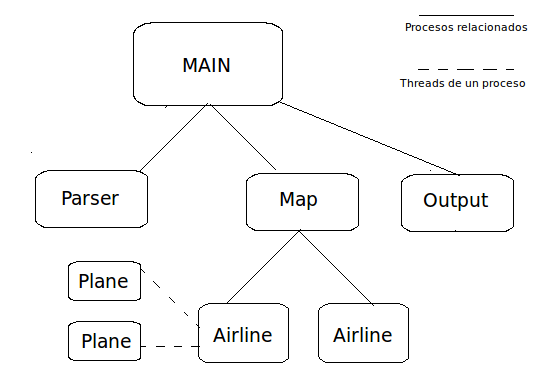
\includegraphics[scale=0.6]{./images/Diagrama_simulacion_2.png}
 % Diagrama_simulacion_2.png: 549x382 pixel, 96dpi, 14.52x10.11 cm, bb=0 0 412 286
 \caption{Esquema inicial de nuestra aplicación.}
\end{center}
\end{figure}


 Luego de cierto debate, vimos que la relación entre el flujo principal, los parsers, el \textit{output} y el mapa era demasiado fuerte, pues, 
 la combinación de estas tres cosas iban a 
 controlar el flujo de la simulación en sí. Inclusive, estas partes tenian una secuencia bastante marcada. Así, se decidió que estos elementos que originalmente bien podrían haber 
 sido planteado como procesos paralelos, era más intuitivo y coherente escribirlo como uno solo.
 Finalmente, el mapa y el \textit{output} fueron implementados como threads del proceso principal ya que si bien su relación es fuerte, nos resulto coherente
  que ambos puedan estar ejecutandose paralelamente. \\

Dado que las aerolineas son independientes entre si, ya que cada una desconoce la existencia de las demas, resulta intuitivo que cada aerolinea ejecute en un proceso dedicado.
Como cada avion es un entidad independiente, pero a la vez es conciente de al existencia del resto de los aviones de su flota, resulta logico que sean threads dentro del proceso de su aerolinea.
Esto nos permite compartir facilmente la informacion que sea necesaria entre aviones, y entre estos y la aerolinea.

\begin{figure}[H]
\begin{center}
 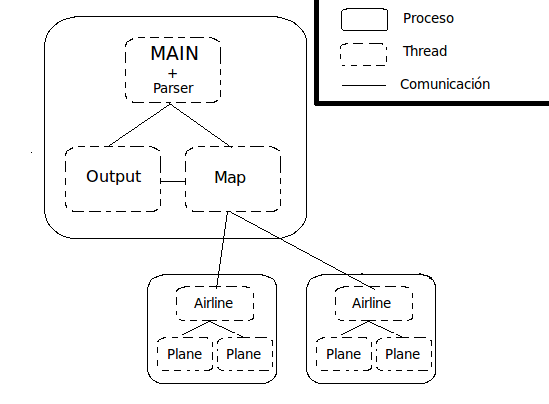
\includegraphics[scale=0.6]{./images/Diagrama_simulacion_1.png}
 % Diagrama_simulacion_1.png: 566x382 pixel, 96dpi, 14.97x10.11 cm, bb=0 0 424 286
 \caption{Esquema final de nuestra aplicación.}
\end{center}
\end{figure}

\newpage
\section{Modelo OSI}

El modelo OSI es un modelo que estandariza la forma de diseñar un programa y como comunicar diferentes programas. 
Este modelo divide una aplicacion en 7 capas, donde cada capa se comunica solo con la capa "debajo".
Esto permite una clara separacion de responsabilidades, llevando a un codigo limpio y facilmente entedible por cualquier familiarizado con el modelo.

El sistema operativo ya provee funcionalidades compatibles con el modelo OSI, con lo cual nuestra implementacion se concierne solo con las 4 capas superiores del modelo.
Para estas 4 capas optamos por desviarnos un poco del modelo, e implementamos las capas de sesion y presentacion en una sola, que llamamos capa de comunicacion.

\begin{figure}[H]
\begin{center}
 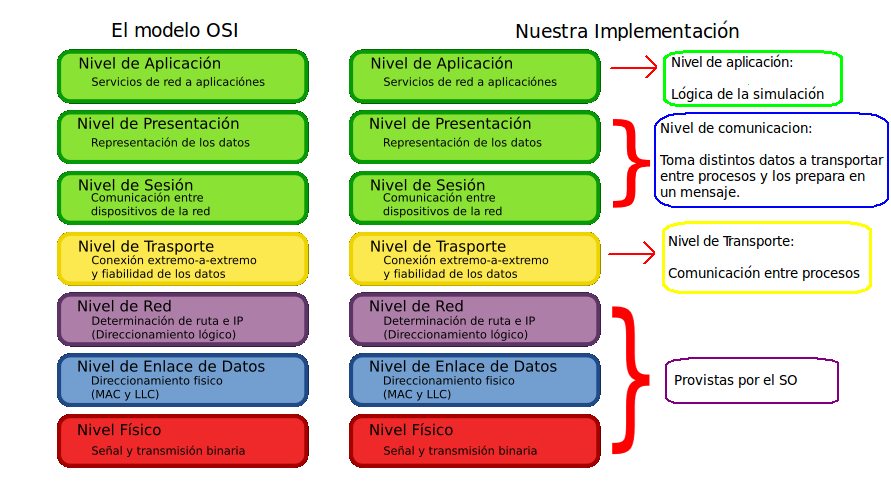
\includegraphics[scale=0.5]{./images/modelo-osi_nuestro.png}
 % modelo-osi_nuestro.png: 891x495 pixel, 96dpi, 23.57x13.10 cm, bb=0 0 668 371
 \caption{Esquema del modelo OSI y nuestra implementación del mismo.}
\end{center}
\end{figure}


\newpage
\section{Transporte}
Uno de los objetivos impuestos era utilizar diversos metodos de comunicacion entre procesos.
La consecuencia natural fue desarrollar una capa de Transporte que soportara todas estas implementaciones.
Para esto diseñamos una interfaz comun a todos los metodos de \textit{IPC}.

Durante el proceso de diseño de la interfaz, pasamos por varios diseños (e implementacion de los mismos) que resultaron deficientes y fueron descartados.
Nuestro primer diseño se baso fuertemente en el comportamiento de la funcion \textit{pipe}, ya que parecia ser la manera mas simple.
O sea, el canal de comunicacion entre 2 procesos se establecia antes de hacer una llamda a \textit{fork}.
Este diseño presenta varias deficiencias, entre ellas que no permite que 2 procesos que no tengan una relacion padre-hijo se comuniquen.
Si bien dado el diseño de nuestra aplicacion esta restriccion es aceptable, detalles de la implementacion complicaban el uso de esta interfaz.
Consecuentemente, por estas complicaciones y limitaciones, optamos por descartar esta interfaz.

Antes de tomar la decision final, evaluamos el uso de una comunicacion bidireccional, donde una conexion permite la salida y entrada de mensajes, o unidireccional.
La comunicacion bidireccional, presentaba la complicacion de necesitar una funcion analoga a \textit{select}.
La implementacion de esta funcion resulto no ser trivial para Shared Memory y Message Queues.
Esto llevo a que descartemos este diseño y nos llevo a nuestro diseño final, una comunicacion unidireccional.

Es un diseño muy parecido al de una Message Queue.
Cada proceso interesado en recibir mensajes, define un nombre unico con el cual indentificarse a la hora de leer mensajes.
Otros procesos pueden escribir mensajes a cualquier otro proceso siempre y cuando sepan bajo que nombre escucha ese proceso.


\newpage
\section{Problemas encontrados(???)}

Uno de los primeros problemas con los que nos topamos, fue el hecho de que los archivos de configuración de los cuales la aplicación debía levantar la información, tenían un formato
bastante díficil para trabajar con el lenguaje C. Al no contar con una estructura que pueda ir agregando elementos a una colección y cambiando de tamaño dinámicamente, debimos 
implementar nuestra propia estructura, \textit{Vector}. Esto probó ser muy útil más adelante ya que la utilizamos en otros sectores del programa.\\

Otro problema con el formato de los archivos de configuración, fue que los límites de las ``iteraciones'' se marcaban con líneas en blanco, y al parecer hay problemas al querer leer el 
$\backslash n$ con $fscanf$. Para lidiar con esta situación, recurrimos a la única solución que encontramos, aunque en términos de código no es muy elegante.\\

Otro problema encontrado, se relaciona con el testeo. Una vez implementadas las 4 implementaciones de la interfaz de IPC, diseñamos un pequeño test inicial, para detectar fallas en una 
etapa temprana. El test no era del todo básico, pero tampoco era muy agresivo. En ese momento, nos concentramos en que las implementaciones efectivamente funcionaran (comunicaran
 procesos). Al no haber hecho un test más exhaustivo, a la hora de testear la aplicación completa como un todo, surguieron algunos pequeños problemas relacionados con la 
 comunicación entre procesos que nuestro test inicial no había logrado detectar.\\

\newpage
\section{Conclusiones}

Queda claro que este trabajo podría haberse realizado sin necesidad de recurrir al procesamiento paralelo y a la comunicación entre procesos. Pero al haberlo 
hecho de de esta forma, la experiencia adquirida y el aprendizaje resulta mucho más significativo. Por varias razones:

\begin{itemize}
\item la experiencia adquirida al trabajar con varios procesos corriendo al mismo tiempo, al igual que varios \textit{threads}.
\item la comunicación entre estos procesos.
\item la separación en capas, consecuencia necesaria, que agrega mucha claridad al código y conceptualmente, al diferenciar claramente las responsabilidades.
\item la familiarización con los estándares \textit{POSIX} y \textit{System V}, o el simple de hecho de trabajar contra interfaces predefinidas y respetando
      un estándar predefinido.
\end{itemize}

Con respecto al uso de \textit{threads}  y procesos, nos topamos con una fuerte diferencia entre utilizar unos y otros. Por ejemplo, el uso de variables globales 
en un \textit{thread} debe ser llevado a cabo con mucho cuidado, ya que el estado global, o \textit{Data Segment}, es compartido por los demás \textit{threads} del mismo
proceso. Esto no es así con los procesos, cuyo estado global es propio y solo visible a ellos mismos. Por suerte, el \textit{stack} no es compartido por distintos \textit{threads}
los que les da un cierto grado de independencia, para que realicen distinas tareas. Otra diferencia que notamos, tiene que ver con la sincronizacíon. Mientras que un
simple \textit{lock} de un \textit{mutex} en la mayoría de los casos era lo único que se debía hacer para sincronizar \textit{threads}, para procesos se requirió el uso
de técnicas más avanzadas como semáforos.

Una vez terminado el trabajo, surgió la pregunta de cual era la implementación de IPC más rápida. Como nos dimos cuenta más tarde, esto no es tan fácil de determinar. 
Esto se debe a que el rendimiento de cada implementación varía dependiendo de la ejecución debido al procesamiento paralelo, el cual no es determínistico. 
Es decir, no siempre se reproduce exactamente la misma ejecución dadas las mismas condiciones iniciales. \\

Para observar la perfomance de la aplicacion, utilizamos 4 simulaciones distintas:

\begin{table}[H]
\begin{center}
\begin{tabular}{l|l|l|l}
Nº & Ciudades & Aerolineas & Aviones \\
\hline
1 & 5 & 2 & 8 \\
2 & 5 & 1 & 3 \\
3 & 10 & 10 & 40 \\
4 & 50 & 10 & 50 \\
\end{tabular}
\caption{Caracteristicas de las simulacions}
\end{center}
\end{table}

Usando estas 4 simulaciones, procedimos a tomar el tiempo de ejecucion de 100 iteraciones consecutivas de cada simulacion.

\begin{figure}[H]
\begin{center}
 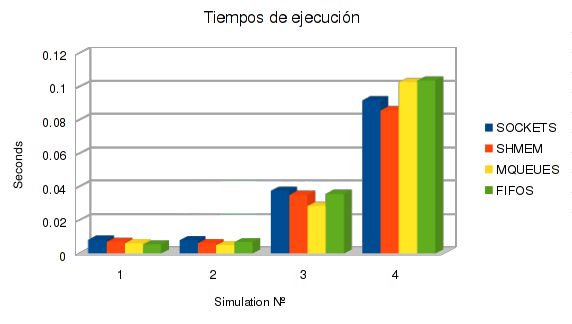
\includegraphics[scale=0.75]{./images/runningTimesChart.png}
 % runningTimesChart.png: 572x324 pixel, 96dpi, 15.13x8.57 cm, bb=0 0 429 243
  \caption{Comparación de los tiempos de ejecución de cada implementación.}
\end{center}
\end{figure}

En base a estos datos, pudimos concluir que en general la de \textit{shared memory} es la implementación con mejores tiempos, seguido de la de \textit{socket}. Aunque,
como puede observarse, para las primeras simulaciones, las menos intensivas, las implementaciones de \textit{message queues} y \textit{fifos} parecen tener mejores tiempos. 
Después de analizar los datos, nuestra explicación es que, en esos casos el mayor \textit{overhead} que tienen las implementaciones como \textit{socket} y 
\textit{shared memory}, hacen que sus tiempos de ejecución sean levemente mayores. 
Pero, para simulaciones más intensivas, como por ejemplo la número 4, ese \textit{overhead} se torna despreciable, revelando los resultados que se observan en el gráfico: esas implementaciones terminan siendo más rápidas.\\

\newpage     
\section{Referencias}

\begin{itemize}
  \item Material provisto por la cátedra.
  \item UNIX system programming. Second Edition. Keith Havilland, Dina Gray, Ben Salama.
  \item http://cplusplus.com/cir
  \item http://beej.us/guide/bgipc/output/html/multipage/unixsock.html
  \item https://computing.llnl.gov/tutorials/pthreads/
  \item https://computing.llnl.gov/tutorials/parallel\_comp/
  \item http://www.csc.villanova.edu/~mdamian/threads/posixsem.html
  \item http://www.cs.cf.ac.uk/Dave/C/node25.html
  \item http://www.users.pjwstk.edu.pl/~jms/qnx/help/watcom/clibref/mq\_overview.html
  \item http://linux.die.net/man/7/mq\_overview
\end{itemize}
   
\end{document}
